\section{Neural Network} %4.6

Unlike random forests, parameters are selected based on out-of-pocket errors in Neural Networks (NN). During the parameter tuning process, k-fold was applied on output testing errors for reference. After multiple tuning, 5 hidden layers were selected. Nine, seven, five, three and one neurons were used in each hidden layer from front to back as Figure \ref{4.2.5-NN-Structure} shown.

\begin{figure}[htbp]
\centering
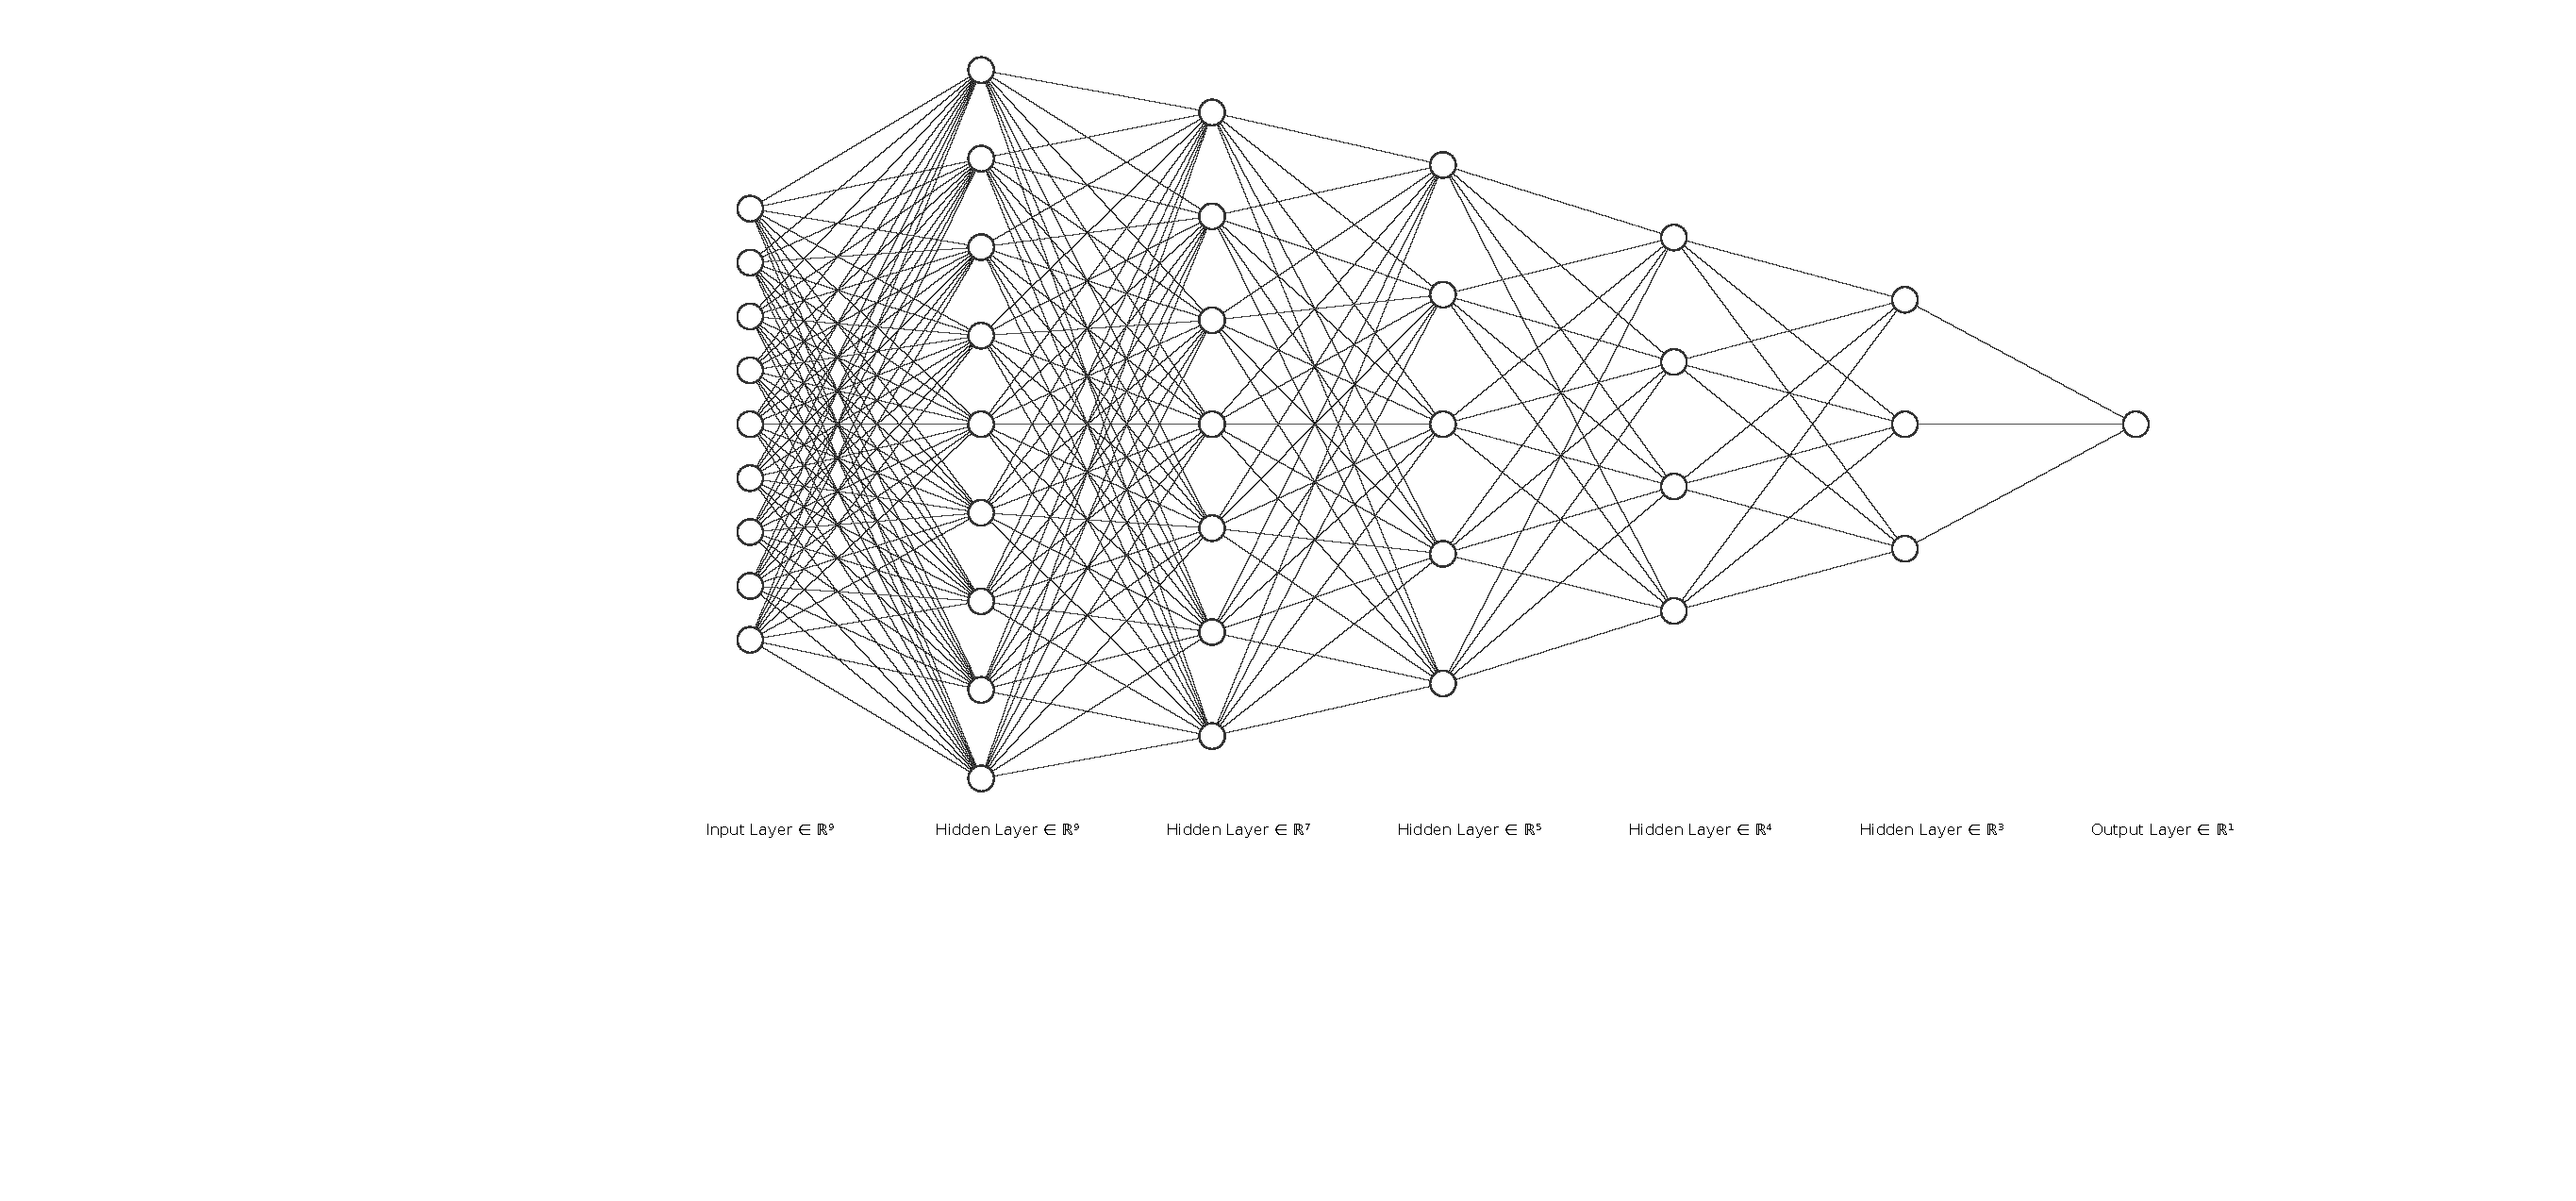
\includegraphics[width = 1.0\textwidth]{Figure/4.2.5-NN-Structure.pdf}
\caption{Neural Networks Structure.}
\label{4.2.5-NN-Structure}
\end{figure}


Similar to Random Forest, the Neural Network algorithm achieved excellent performance. The MSE value of Neural Network was slightly higher than the Random Forest, reaching 0.00106. The fitting diagram (right of Figure \ref{4.2.5-NN}) also proves that the variance of the Neural Networks model is very low comparing with previous Supervised Learning algorithms excluding Random Forest.


\begin{figure}[htbp]
\centering
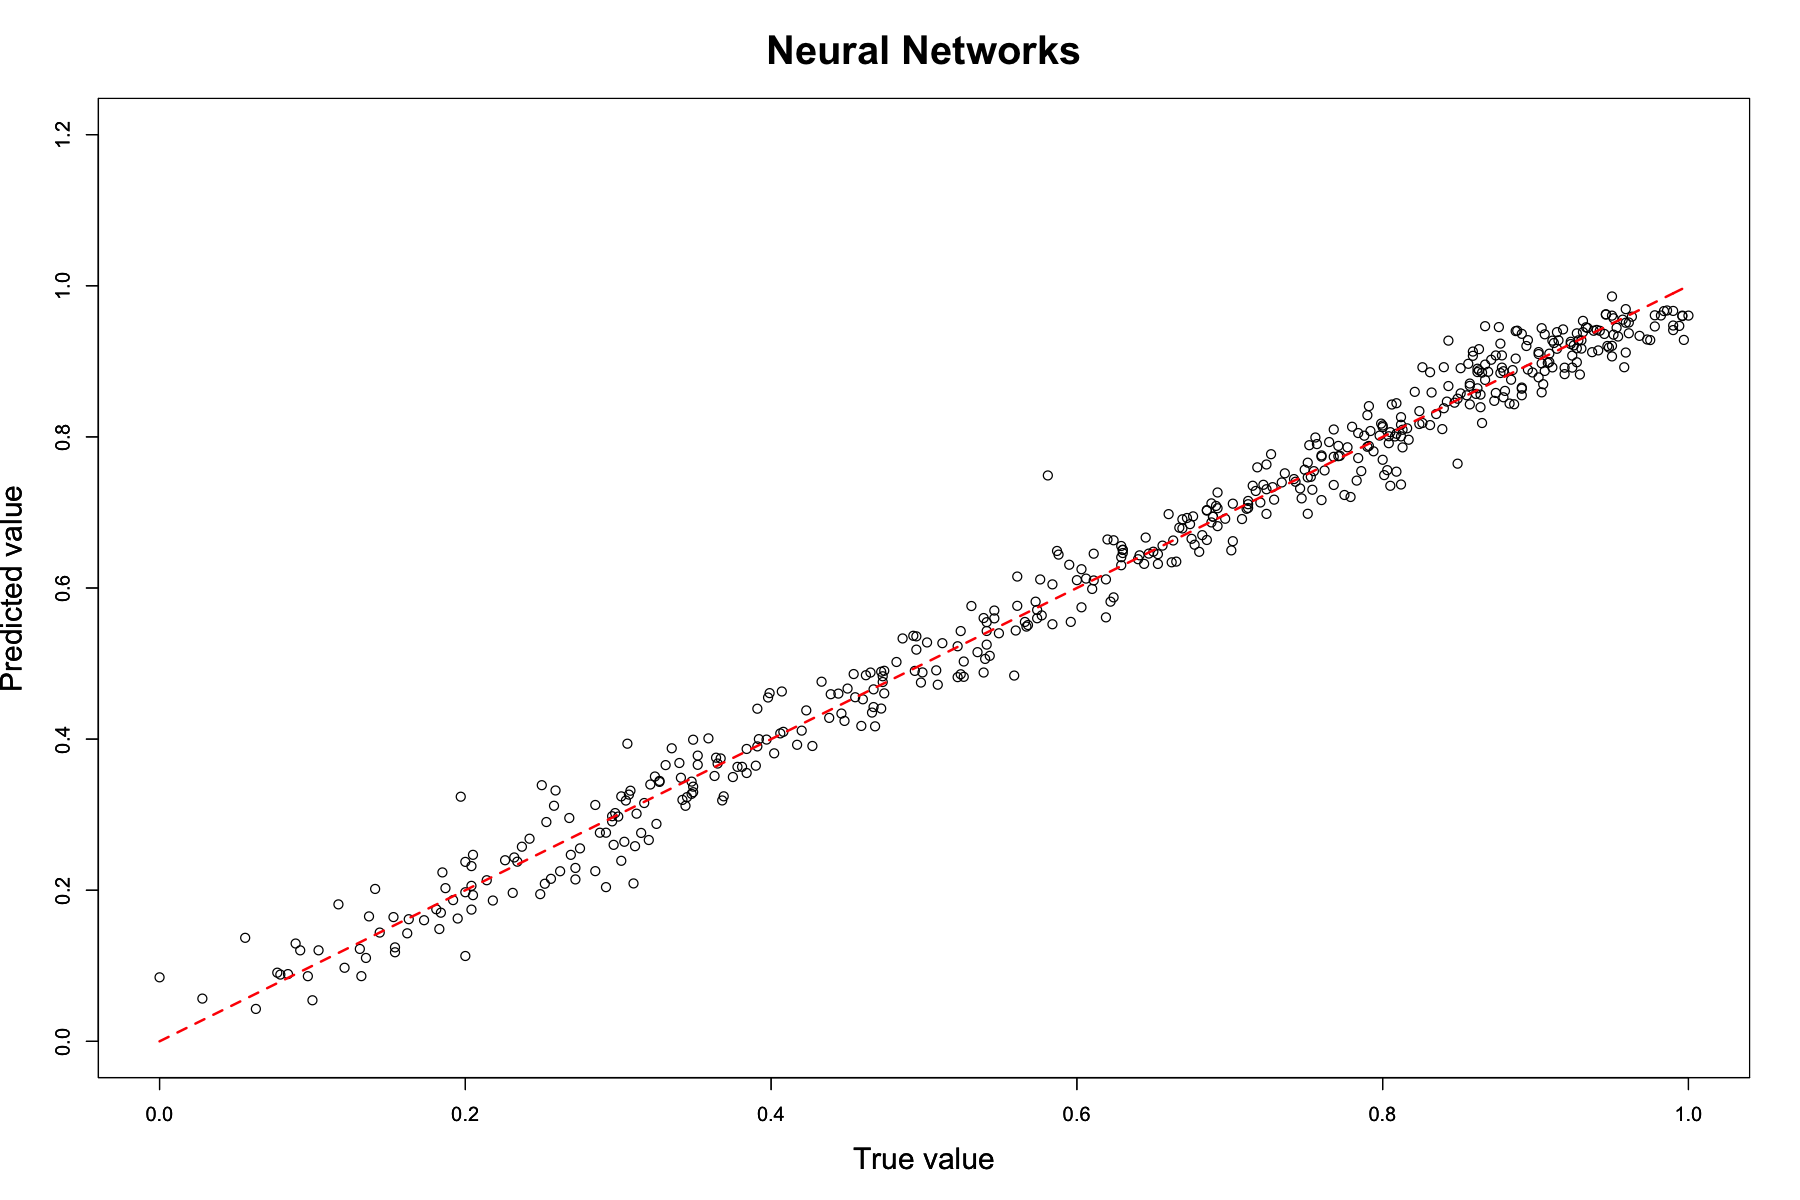
\includegraphics[width = 1.0\textwidth]{Figure/4.2.5-NN.png}
\caption{The predicted Arctic sea ice extent value vs the real Arctic sea ice extent value with \textbf{Neural Networks} (9 neurons, 5 hidden layers with (9,7,5,4,3) nodes respectively). The red referenced dotted line represents the straight line y=x. Mean Square Error (MSE) is \textbf{0.00106}.}
\label{4.2.5-NN}
\end{figure}


\newpage